\section{results}\label{sec:results}
\subsection{Generation results}\label{subsec:generation-results}
The results were made by measuring the generation time for a \gls{void} description for different database sizes. The database started at 1 million triples and was incremented by 10,000 triples up to 10,000,000. A \gls{void} description was generated for each increment for the database, and the time it took to generate it was measured in ms by the "time" library in Python. This was done ten times to ensure the results would be reliable. From this, a graph could be made, and a linear regression could be made to show the trend of the generation time. This helps to show how much the time to generate a \gls{void} description increases as the database size increases.

A graph of the standard deviation of the results can be seen in \autoref{fig:generate-dbsize-all}, which shows the size of the database along the x-axis and the generation time in ms on the y-axis. Each point in the graph has a span, the standard deviation of the results. From the graph, it is clear that there is a trend that the data follows. As the database size increases, so does the time it takes to generate a \gls{void} description; the time increases linearly with the database size.

\begin{figure}[htb!]
    \centering
    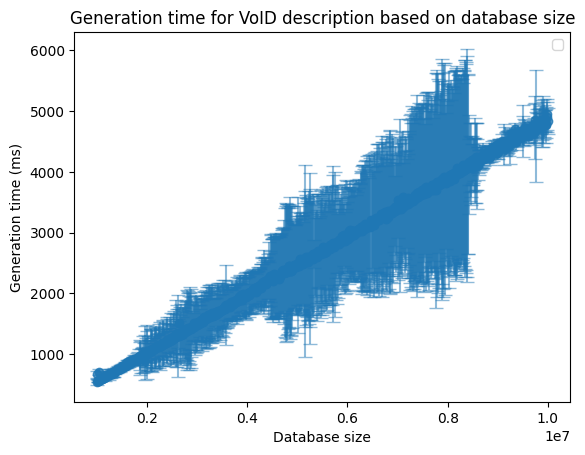
\includegraphics[width=0.8\columnwidth]{figures/generation-results-graph.png}
    \caption{2D graph showing the standard number of tripels impact of database size on the time it takes to generate a \gls{void} description. Containing all the data.}
    \label{fig:generate-dbsize-all}
\end{figure}

Though there is a strange trend when the database reaches the size above 8,000,000 triples, the standard deviation of the results suddenly decreases. To better understand why this happens, we can show a graph over all ten runs and see if anything could indicate why the sudden decrease happens. In \autoref{fig:generate-dbsize-10-runs-all}, we can see the results of all ten runs.

\begin{figure}[htb!]
    \centering
    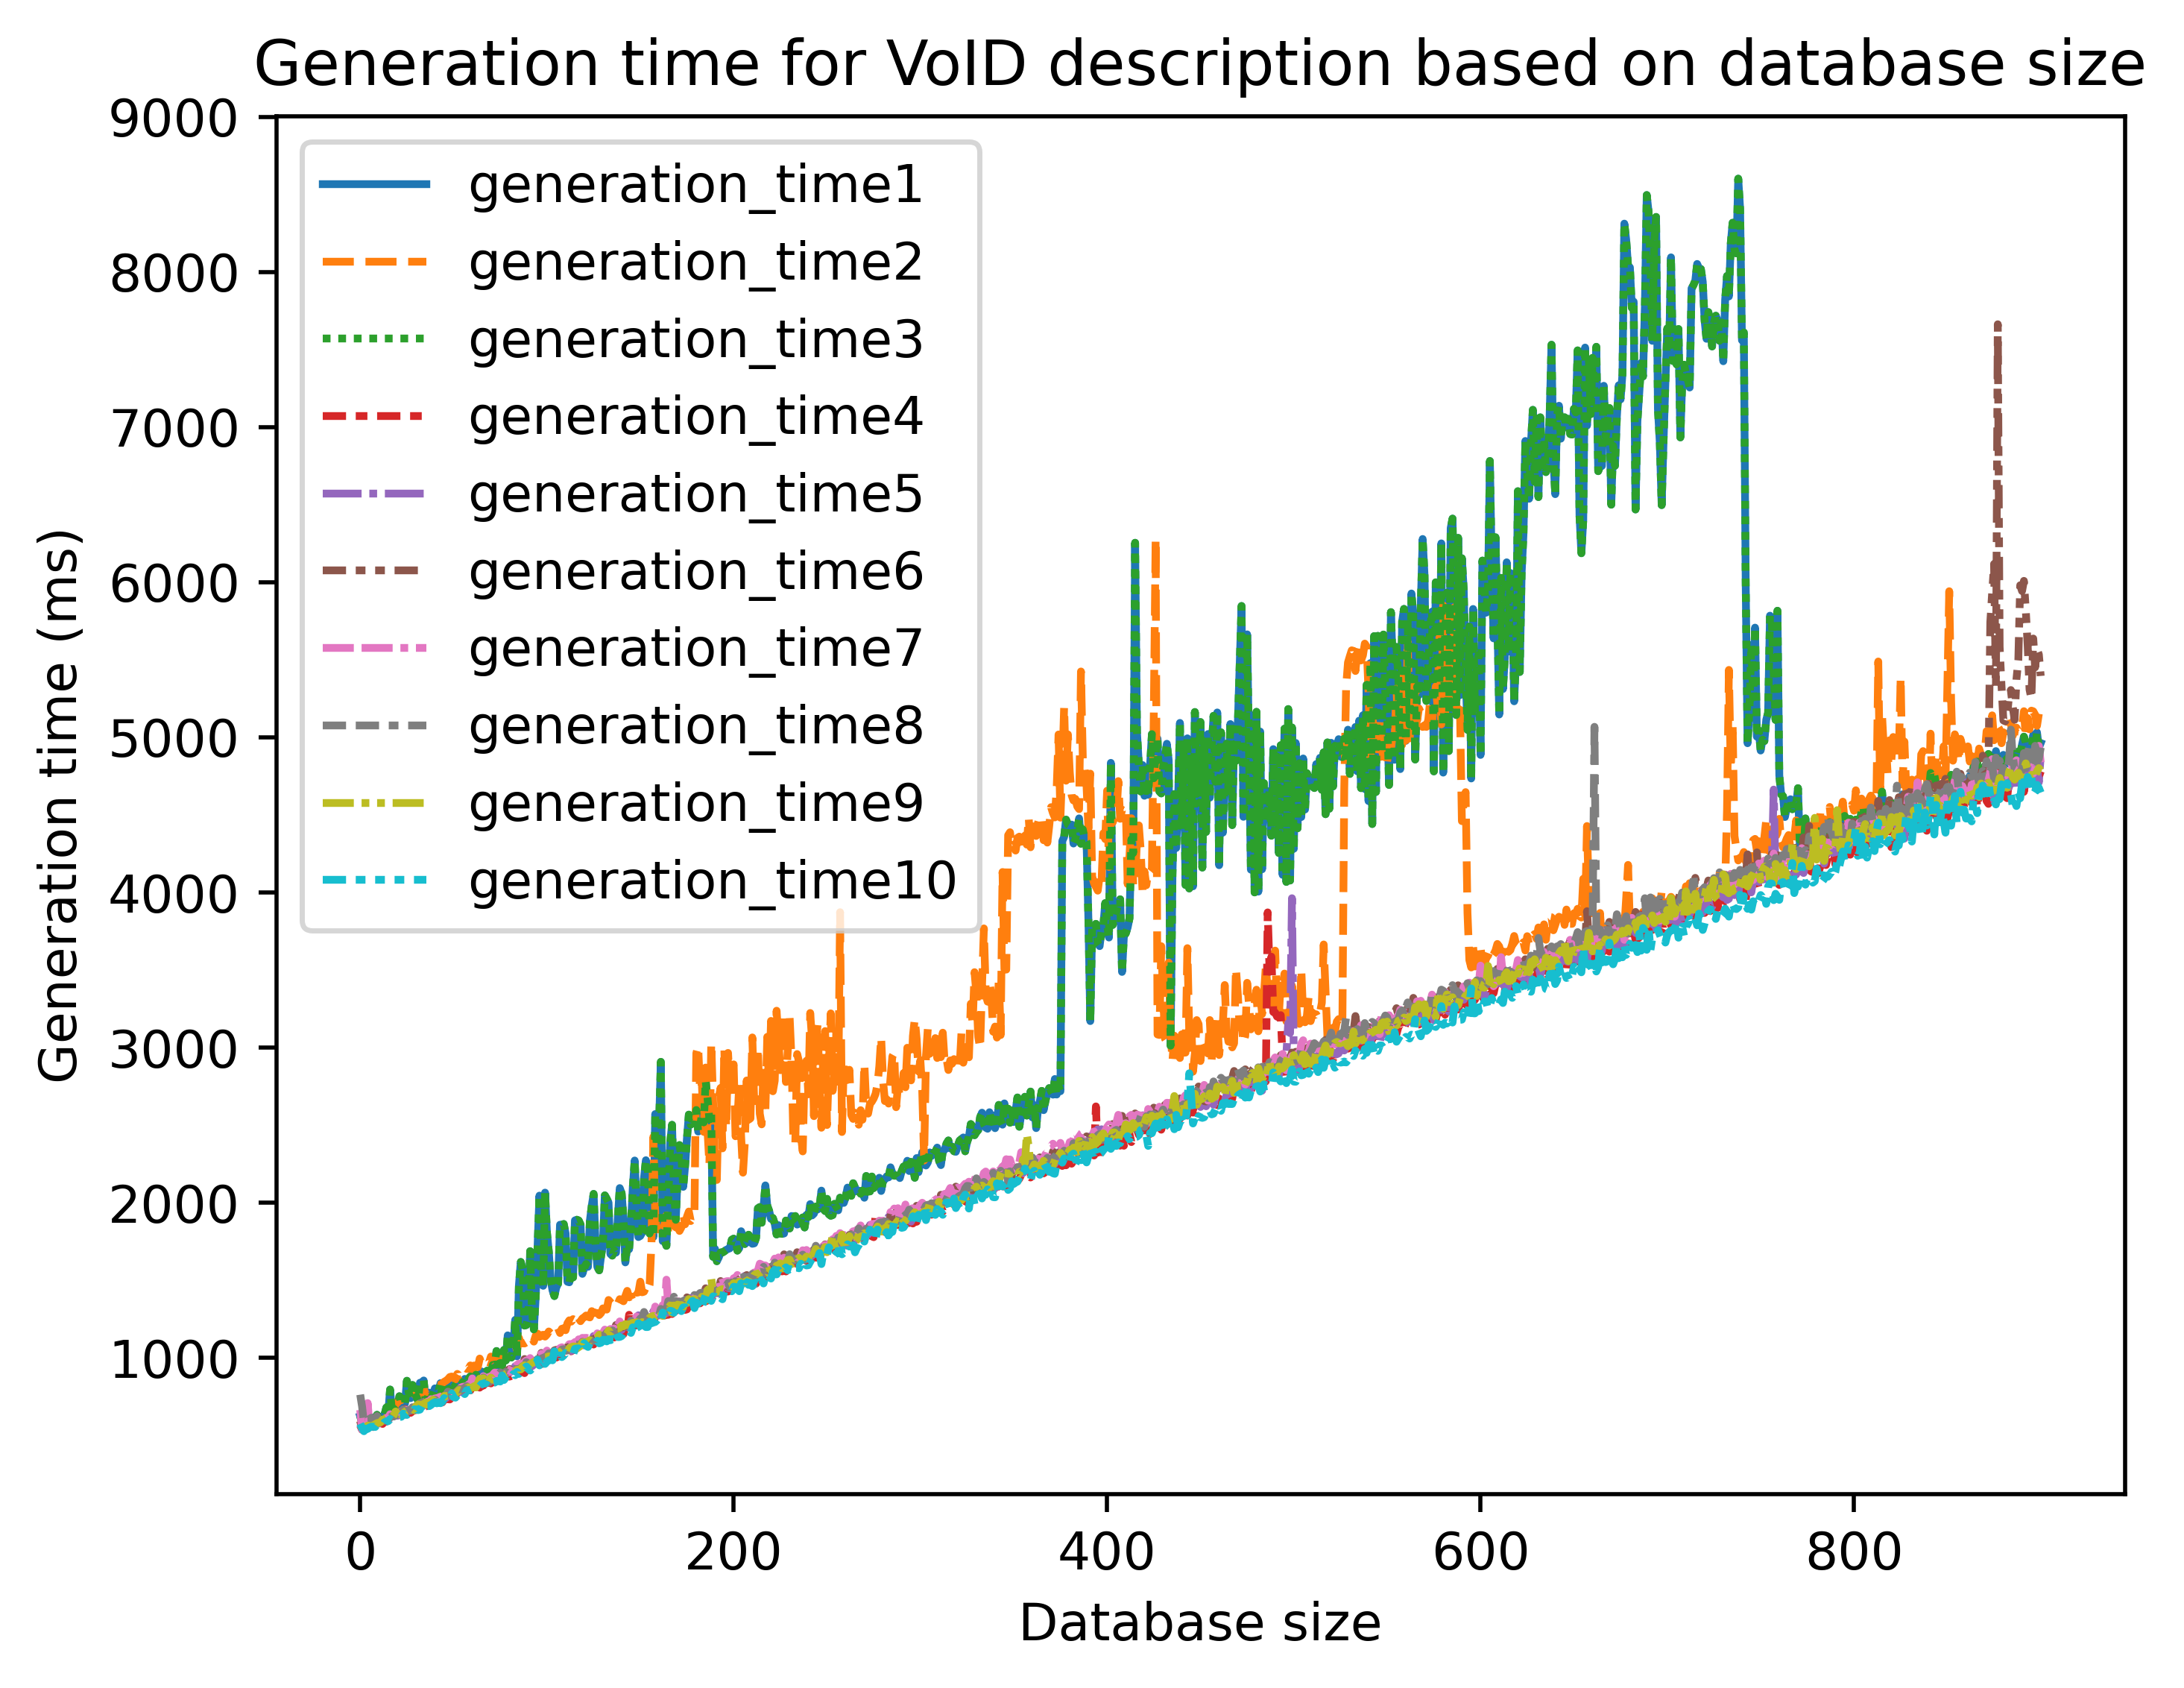
\includegraphics[width=0.8\columnwidth]{figures/generation-results-graph-all.png}
    \caption{2D graph showing each runs impact of database size on the time it takes to generate a \gls{void} description. Containing all the data.}
    \label{fig:generate-dbsize-10-runs-all}
\end{figure}

Certain outliers deviate significantly from others. This is most likely because the computer running the measurements was in use during the first few runs. This has likely affected the results and caused the outliers. This can be even more seen when sorting these outliers out in \autoref{fig:generate-dbsize-10-runs-good}. In this graph, all the results are much more similar, showing that, when generating the results, it was susceptible to any other activity happening on the machine, thereby creating outliers. So by generating a new graph with the outliers removed, we can see that the standard deviation of the results is much more stable and still follows the same trend as before.

\begin{figure}[htb!]
    \centering
    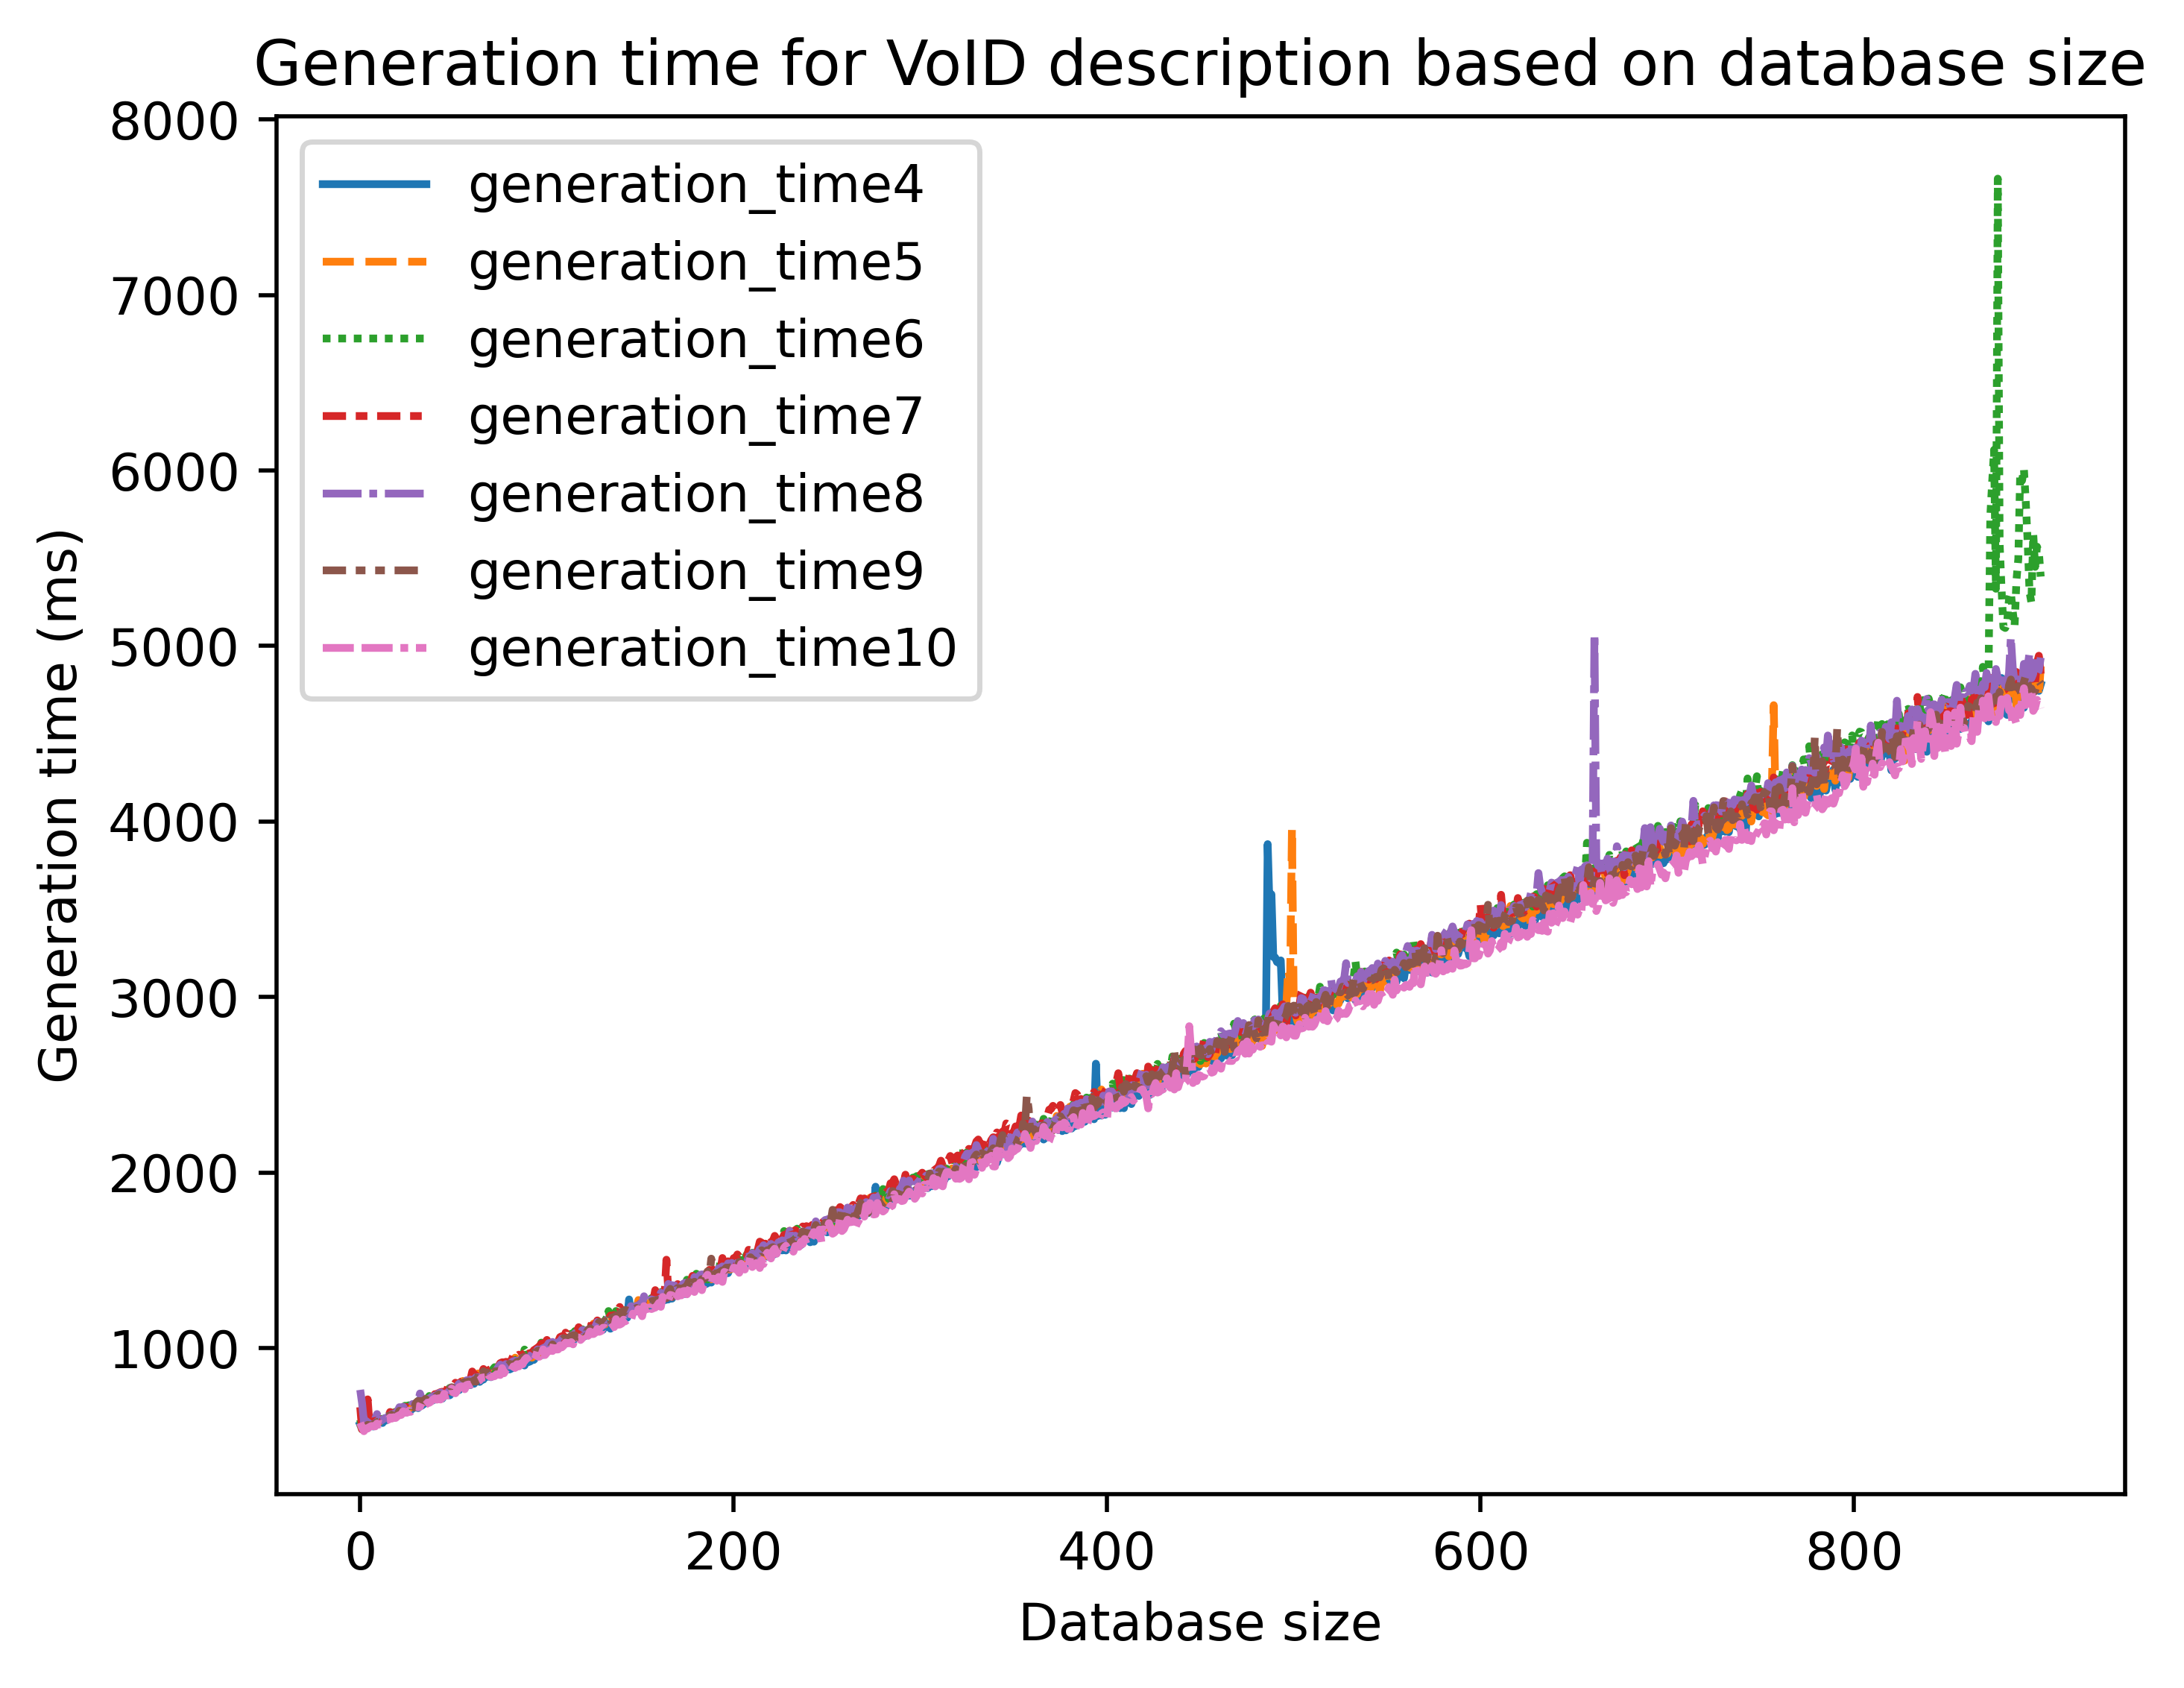
\includegraphics[width=0.8\columnwidth]{figures/generation-results-graph-all-good.png}
    \caption{2D graph showing each runs impact of database size on the time it takes to generate a \gls{void} description. Containing only the good data.}
    \label{fig:generate-dbsize-10-runs-good}
\end{figure}

From this, we can gather that the time it takes to generate a \gls{void} description for a database linearly increases as the database size increases. This is expected because the script only processes the triples in the database, and the more triples there are, the more triples the script has to process. This means that the time it takes to generate a \gls{void} description is directly proportional to the number of triples in the database.

\subsection{Update results}\label{subsec:update-results}
The results for updating the \gls{void} description contained three parameters: time, query size, and database size. The query size was measured when updating the \gls{void} description but not when generating it because query size did not affect generation, as the generation is purely based on what is in the database.

The results were made by measuring the time it took to update the \gls{void} description for database and query sizes. As in \autoref{subsec:generation-results}, the database started at 1 million triples and incremented by 10,000 triples up to 10,000,000. The difference is that query size is simulated by creating a query of one triple and incrementing it by 1,000 up to 8,001, whereafter, the database size is incremented by 10,000.

The query size ended at 8,001 because when the query size was more than 10,000 triples, the query could fail due to unknown reasons. Therefore it was decided to stop at 8,001 triples, as the queries were still large enough to show the trend of the update time.

The generation results were measured in increments of 10,000, where the \gls{void} description was generated and the generation time was measured.

The update results were measured nine times for every 10,000 increments of the database size with different query sizes. The query size for each iteration started at one and was incremented by 1,000 up to 8,001. This means the update results have nine times more data than the generation results.

As with \autoref{subsec:generation-results}, the computer used during the measurements impacted the first three runs. This can be seen in \autoref{fig:update-querysize-all}, where some outliers deviate significantly from the rest of the data. Because of the outliers, we are mainly interested in the data generated without the computer being used, as this data is more reliable, as seen in \autoref{fig:update-querysize-good}.

\begin{figure}[htb!]
    \centering
    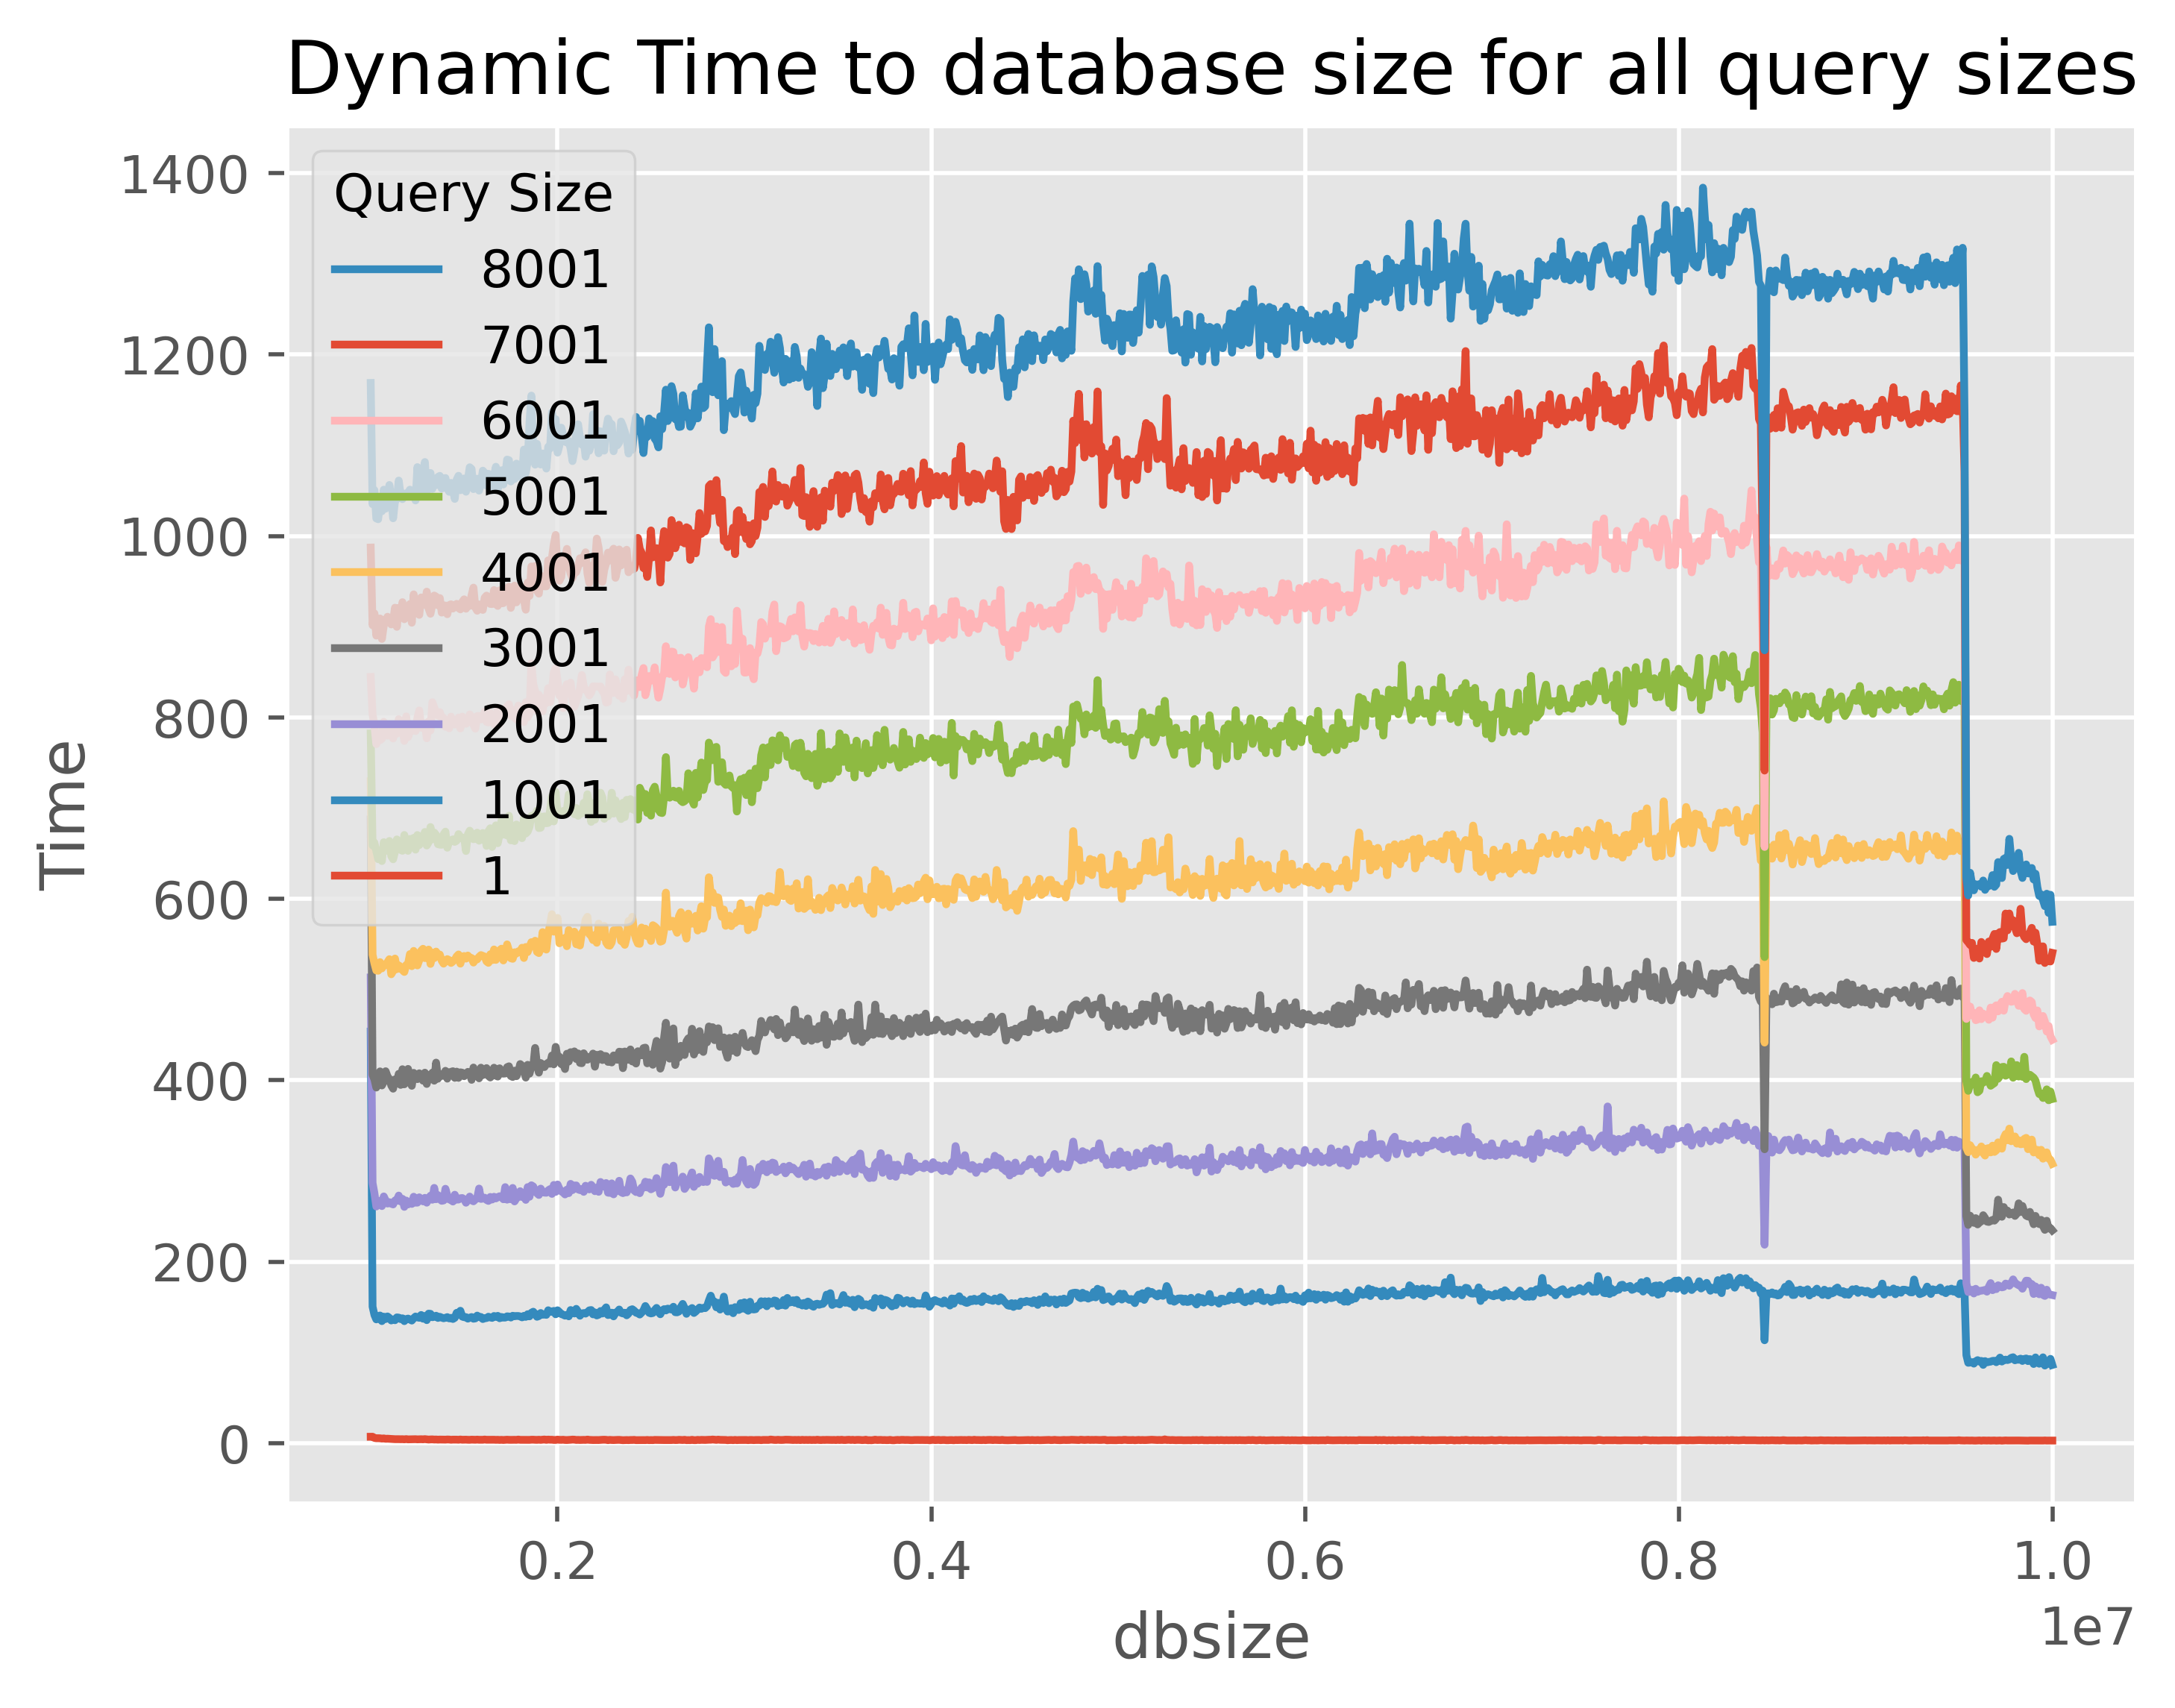
\includegraphics[width=0.8\columnwidth]{figures/dynamic-time-query-size-all.png}
    \caption{2D graph showing the impact of query size and database size on the time it takes to update a \gls{void} description, containing all the data.}
    \label{fig:update-querysize-all}
\end{figure}

\begin{figure}[htb!]
    \centering
    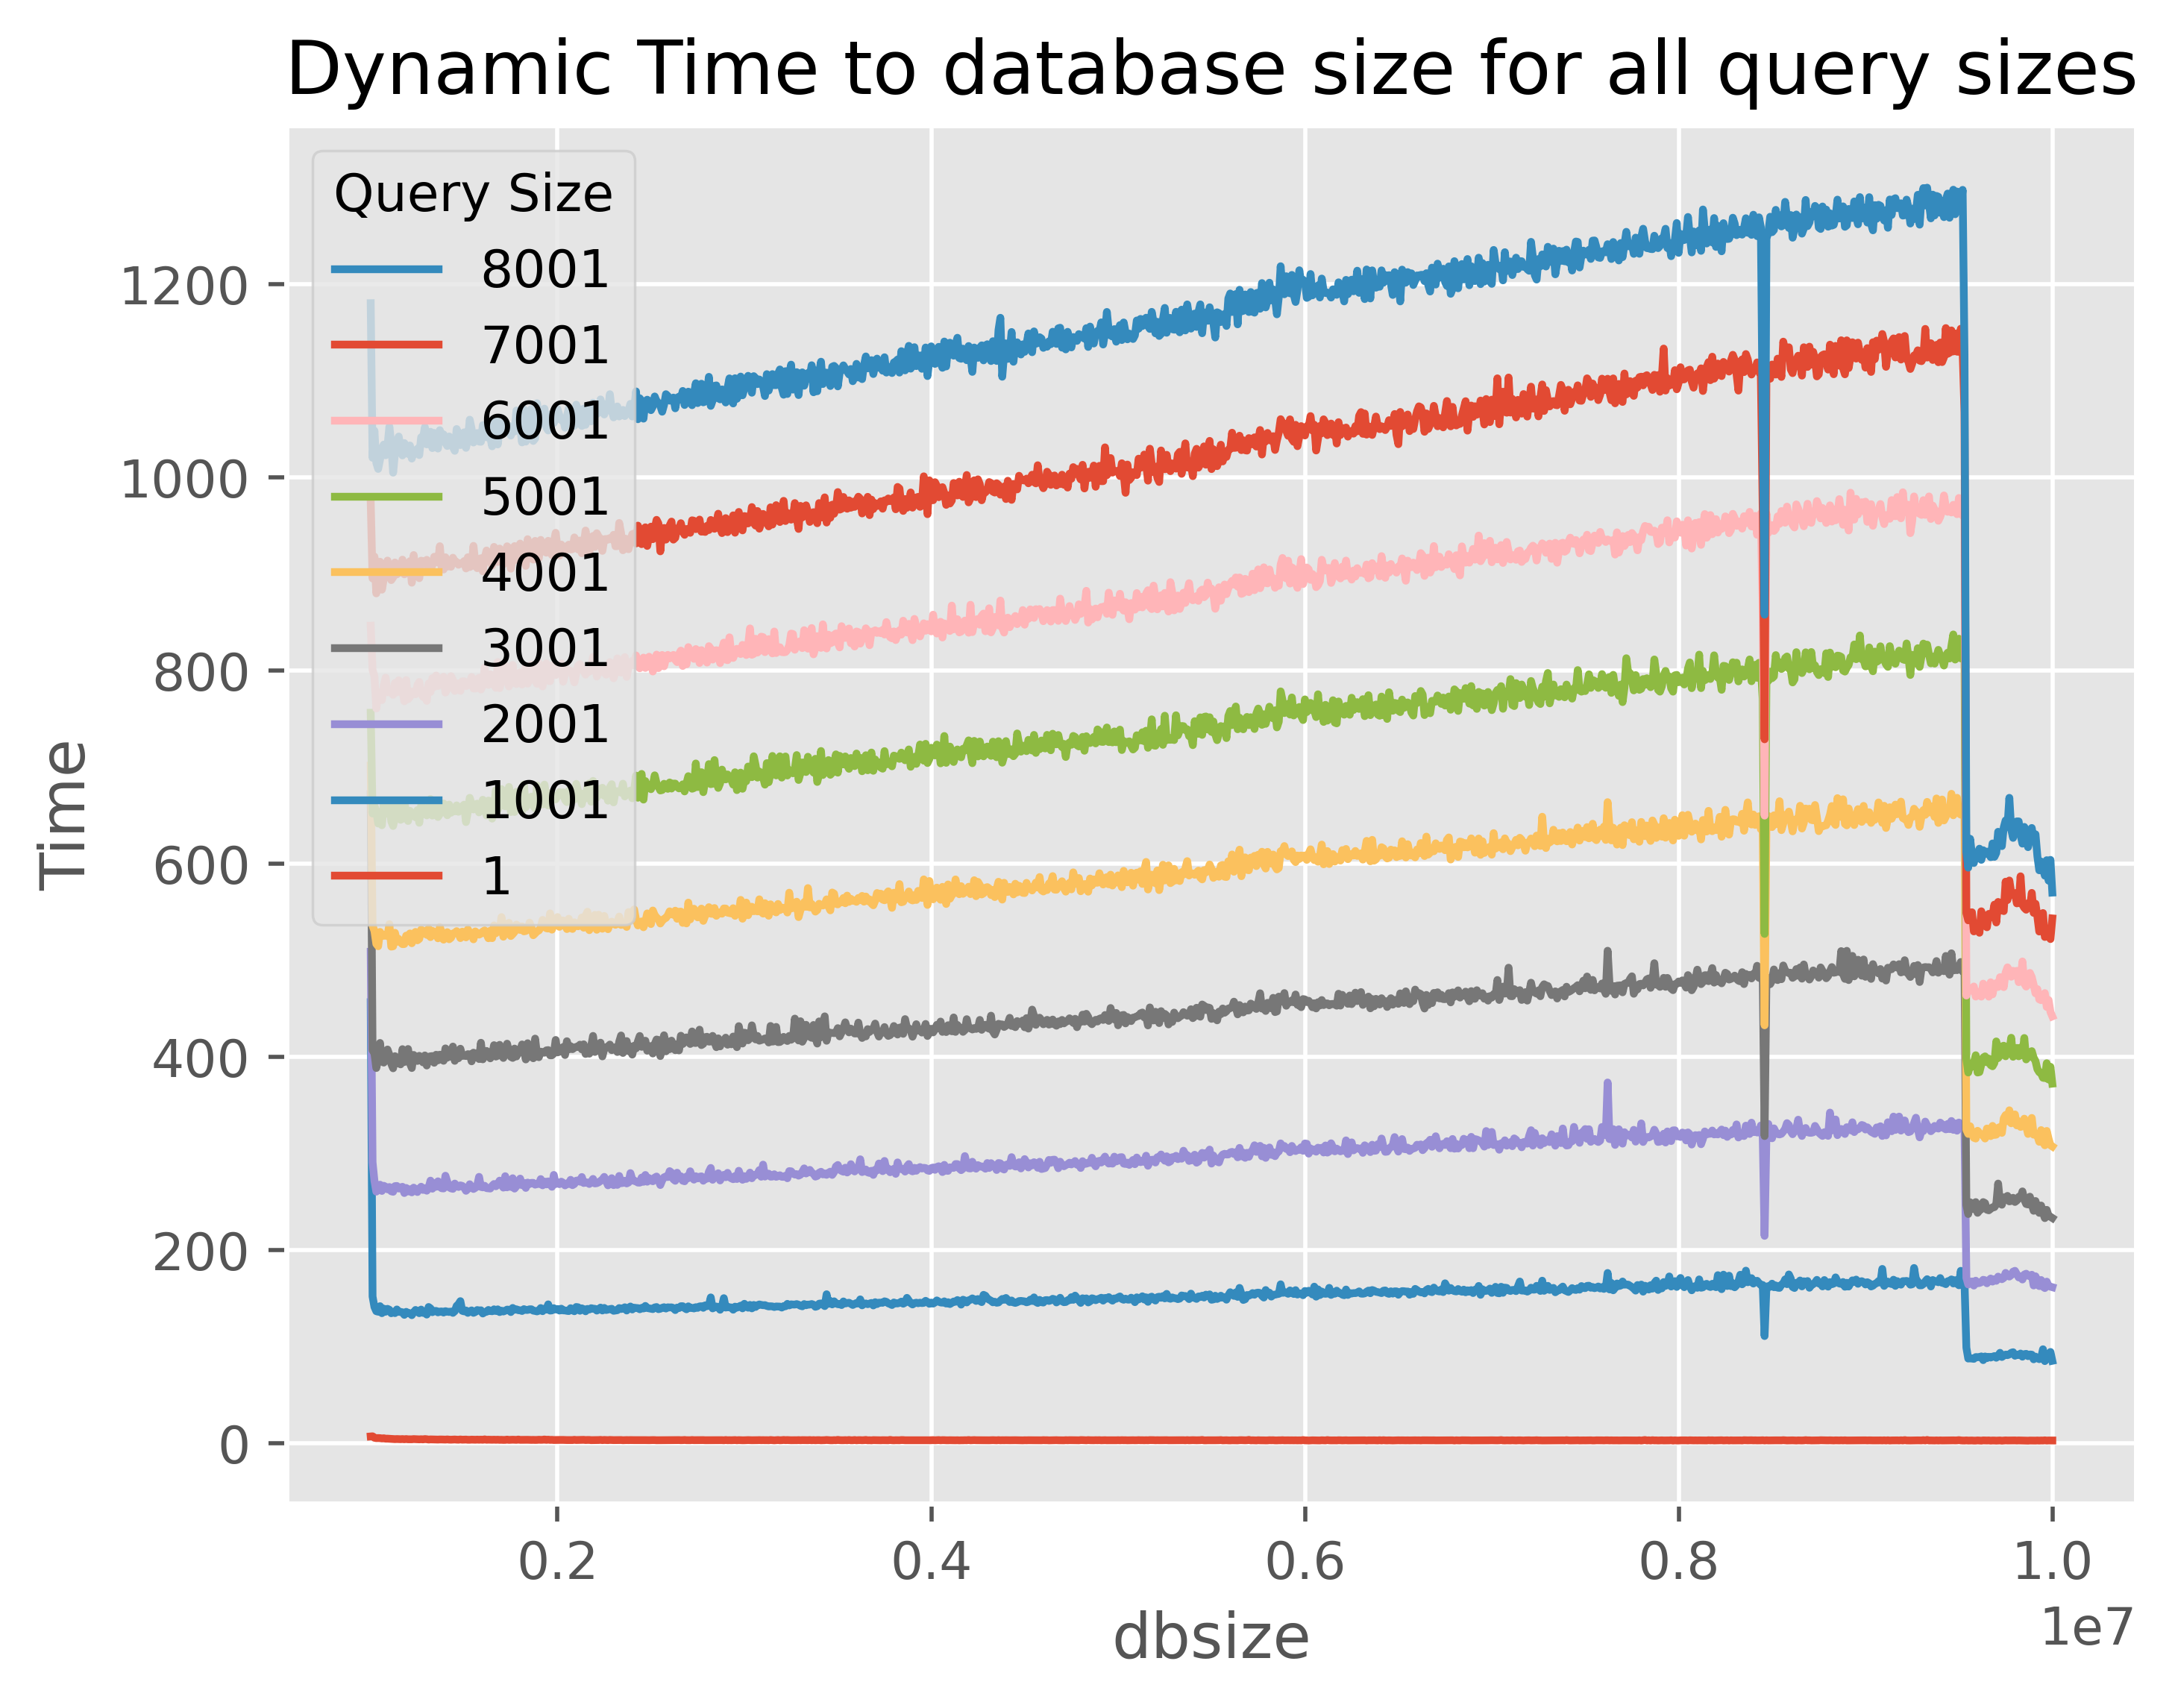
\includegraphics[width=0.8\columnwidth]{figures/dynamic-time-query-size-good.png}
    \caption{2D graph showing the impact of query size and database size on the time it takes to update a \gls{void} description, containing only the good data.}
    \label{fig:update-querysize-good}
\end{figure}


The 2D-graph in \autoref{fig:update-querysize-good} shows the impact of query size and database size on the time it takes to update a \gls{void} description. From this graph, it is clear to see that there is a trend that the data follows.

The query size significantly impacts the time it takes to update the \gls{void} description, and the database size bearly impacts the time it takes to update the \gls{void} description. This is because as the amount of new data inserted into the database increases, so does the time to update the \gls{void} description because the script has to process more data. However, all the data inserted is new, meaning it is currently unknown if updating existing data will significantly impact the time it takes to update the \gls{void} description.

This could be tested in the future, but it will likely not significantly impact the time it takes to update the \gls{void} description. This is because the script does not have to process the data already in the database; therefore, it will not impact the time it takes to update the \gls{void} description. However, if this is the case, it has yet to be discovered, and it could be tested in the future.

A 2D graph clearly displayed the impact of database size and query size. In \autoref{fig:update-querysize-good}, we can see that the database size has a minor effect on the time to update, but the query size is the main factor in the time it takes to update the \gls{void} description.

There is an unexpected trend in the graph, where the time it takes to update the \gls{void} description suddenly decreases when the database is almost 10,000,000 triples. The decrease in time to update the \gls{void} description did not appear to be directly related to the number of triples inserted. However, upon examining the inserted data, which can be seen in \autoref{lst:inserted-data-start} and \autoref{lst:inserted-data-end}, it was observed the density of the data was significantly lower than the previous data, as there were many more triples with literal objects than at the start.

\begin{listing}
    \begin{minted}{turtle}
        http://db.uwaterloo.ca/~galuc/wsdbm/User67000    http://db.uwaterloo.ca/~galuc/wsdbm/friendOf    http://db.uwaterloo.ca/~galuc/wsdbm/User90005 .
http://db.uwaterloo.ca/~galuc/wsdbm/User67000    http://db.uwaterloo.ca/~galuc/wsdbm/friendOf    http://db.uwaterloo.ca/~galuc/wsdbm/User91840 .
http://db.uwaterloo.ca/~galuc/wsdbm/User67000    http://db.uwaterloo.ca/~galuc/wsdbm/friendOf    http://db.uwaterloo.ca/~galuc/wsdbm/User93344 .
http://db.uwaterloo.ca/~galuc/wsdbm/User67000    http://db.uwaterloo.ca/~galuc/wsdbm/friendOf    http://db.uwaterloo.ca/~galuc/wsdbm/User9477 .
http://db.uwaterloo.ca/~galuc/wsdbm/User67000    http://db.uwaterloo.ca/~galuc/wsdbm/friendOf    http://db.uwaterloo.ca/~galuc/wsdbm/User94912 .
\end{minted}
    \caption{Example of the inserted data that at the start.}
    \label{lst:inserted-data-start}
\end{listing}

\begin{listing}
    \begin{minted}{turtle}
    http://db.uwaterloo.ca/~galuc/wsdbm/Purchase132942    http://purl.org/goodrelations/price    "824" .
    http://db.uwaterloo.ca/~galuc/wsdbm/Purchase132943    http://db.uwaterloo.ca/~galuc/wsdbm/purchaseFor    http://db.uwaterloo.ca/~galuc/wsdbm/Product732 .
    http://db.uwaterloo.ca/~galuc/wsdbm/Purchase132943    http://purl.org/goodrelations/price    "368" .
    http://db.uwaterloo.ca/~galuc/wsdbm/Purchase132944    http://db.uwaterloo.ca/~galuc/wsdbm/purchaseDate    "2012-09-17" .
    http://db.uwaterloo.ca/~galuc/wsdbm/Purchase132944    http://db.uwaterloo.ca/~galuc/wsdbm/purchaseFor    http://db.uwaterloo.ca/~galuc/wsdbm/Product1 .
    http://db.uwaterloo.ca/~galuc/wsdbm/Purchase132944    http://purl.org/goodrelations/price    "845" .        
\end{minted}
    \caption{Example of the inserted data that at the end.}
    \label{lst:inserted-data-end}
\end{listing}

This suggests that the data structure significantly affects the time required for updating the \gls{void} description. However, which specific aspects of the data are primarily responsible for this effect remains unclear. For example, factors such as the number of characters, data type, or other variables could contribute to the decrease in update time. Investigating how the data's structure influences the time needed to update the \gls{void} description would be an intriguing area for future research.

From these findings, we can gather that the time it takes to update a \gls{void} description is heavily impacted by the size of the query (the number of characters in the query) that is being inserted and not so much the size of the database.


\subsection{Update and generation comparison}\label{subsec:update-generation-comparison}
\autoref{fig:comparison-generation-vs-update} shows a 2D graph of the impact of database size on the time it takes to generate a \gls{void} description and the time it takes to update a \gls{void} description. Since generating a \gls{void} description is greatly affected by the size of the database, the time it takes to generate a \gls{void} description increases significantly faster than the time it takes to update a \gls{void} description.

In comparison, the database size barely affects the nine update measurements for each query size. From this, it can be gathered that the larger the database is, the more it makes sense to update the \gls{void} description instead of generating it from scratch, but with a smaller database, it makes more sense to generate the \gls{void} description from scratch.

\begin{figure*}[t]
    \centering
    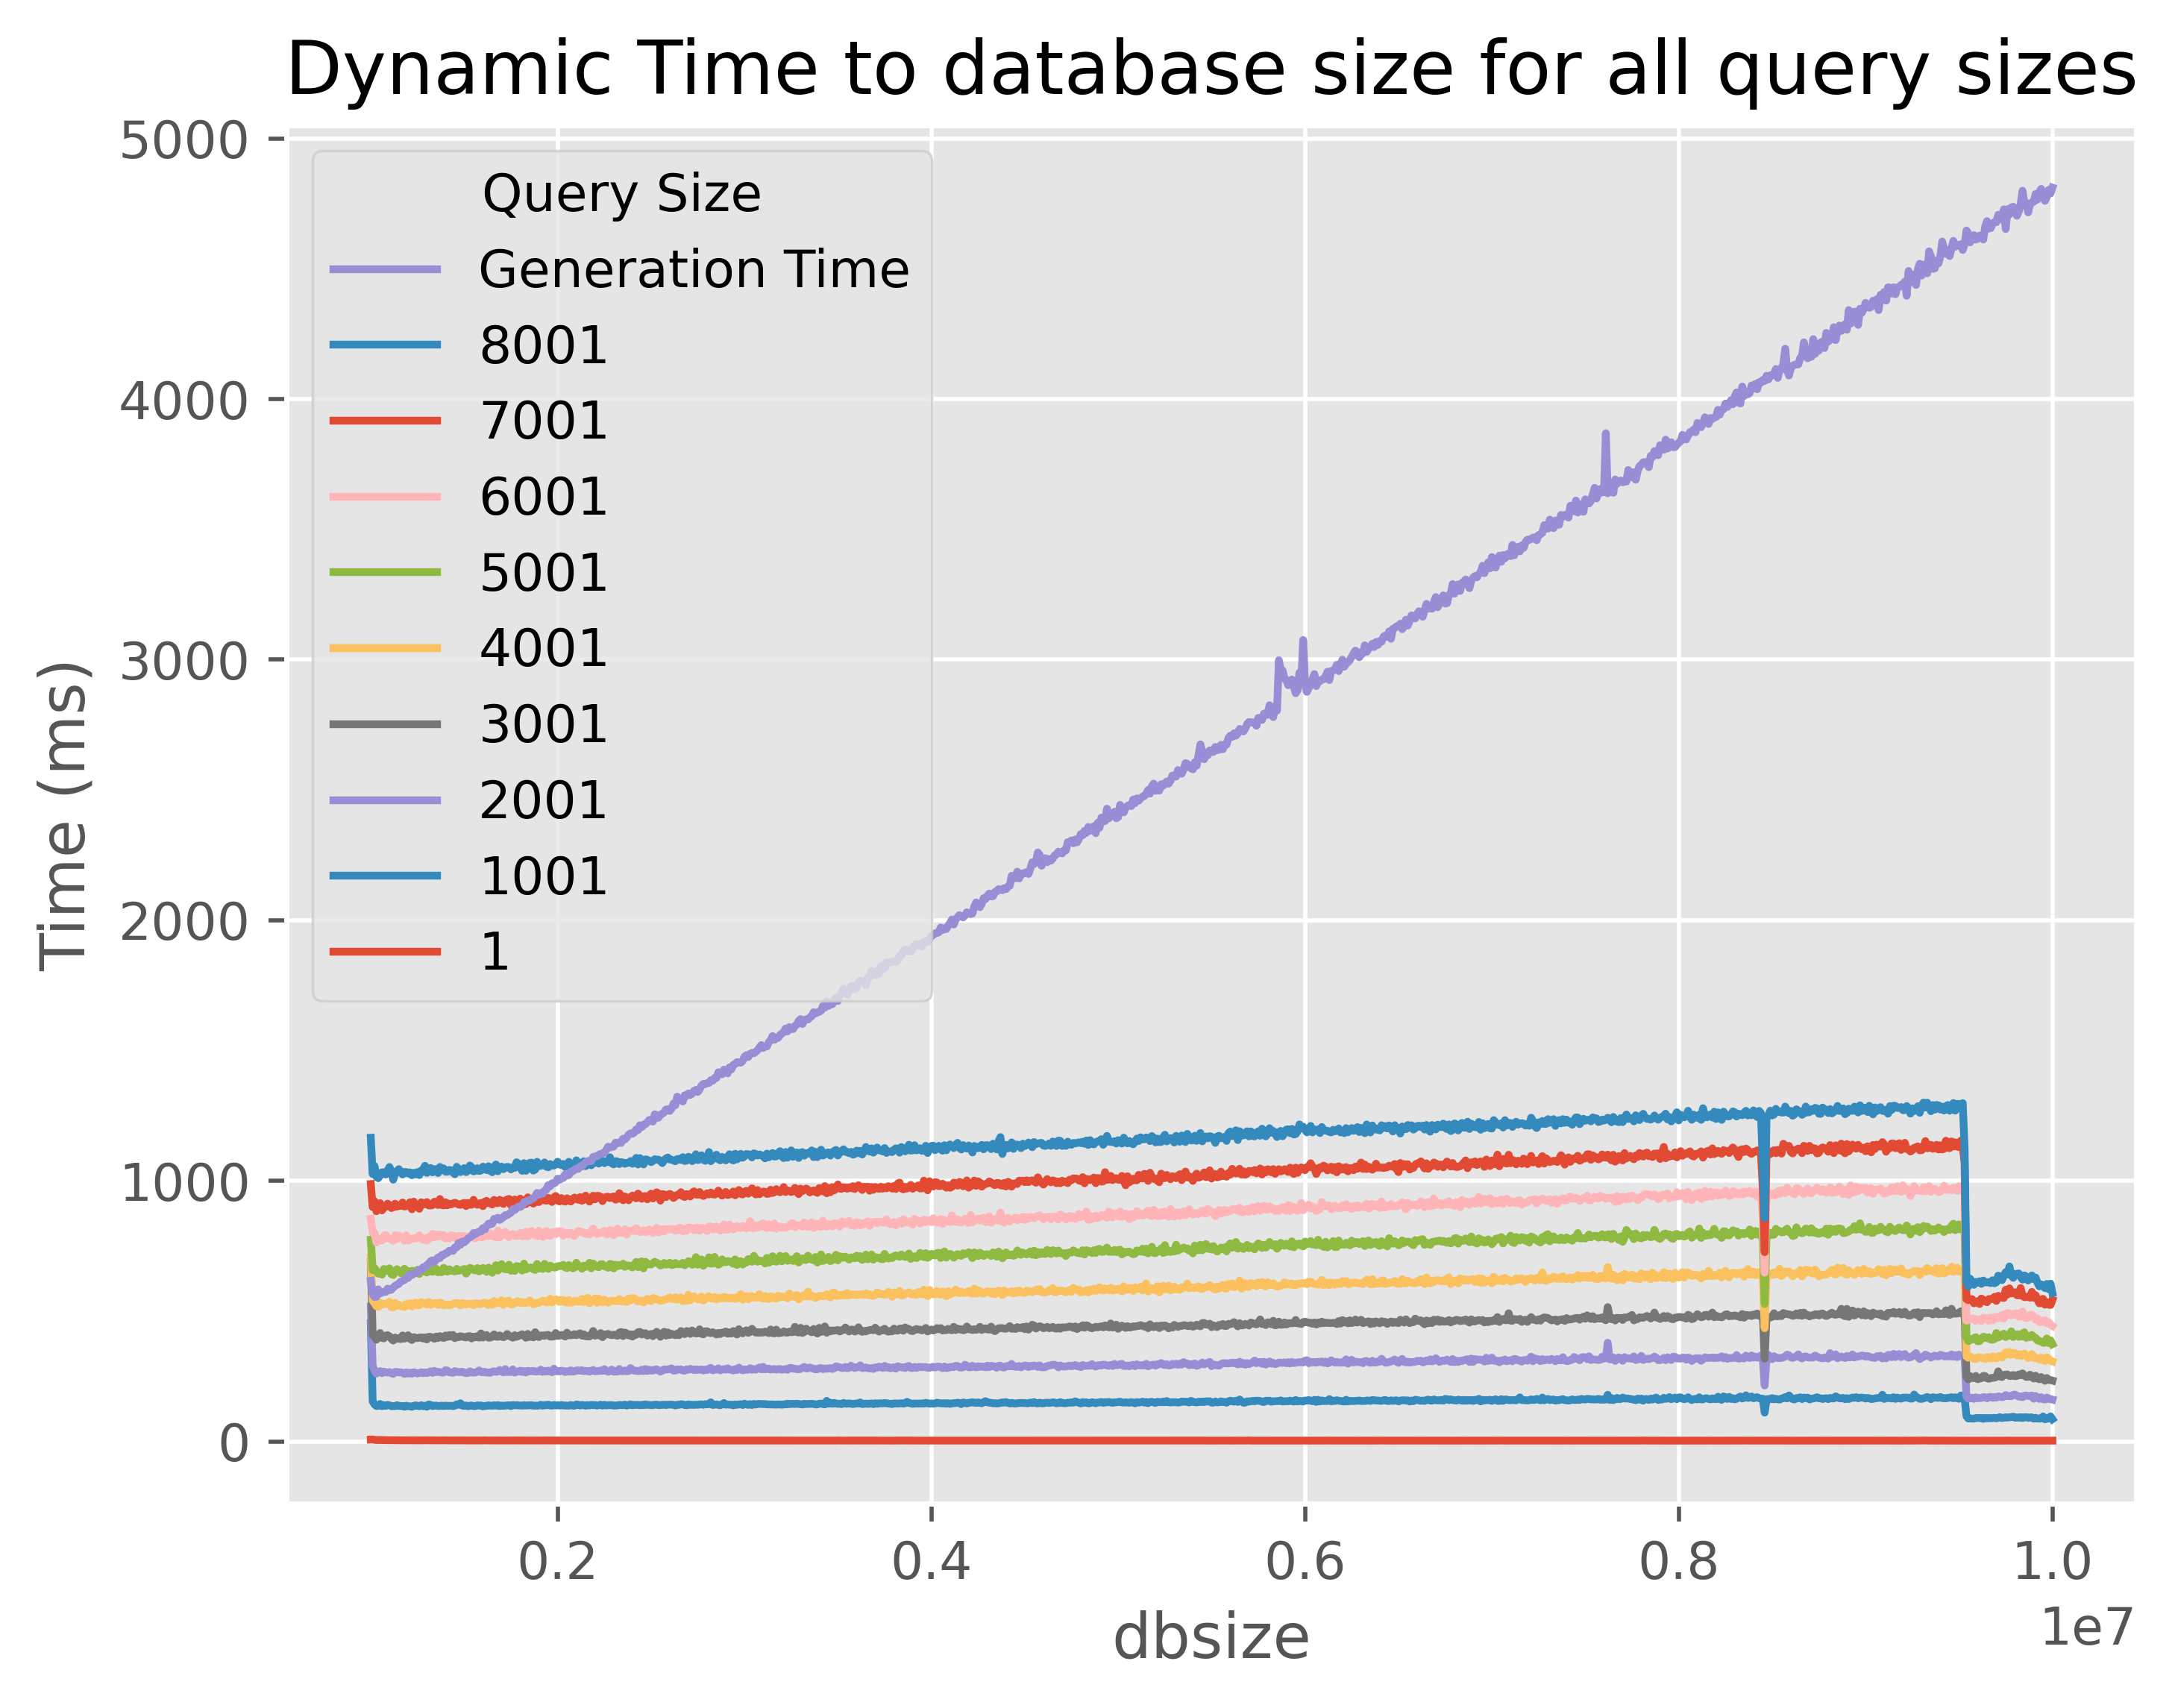
\includegraphics[width=0.8\textwidth]{figures/comparison-Generation-vs-Update.png}
    \caption{Comparison between the time it takes to generate a \gls{void} description and the time it takes to update a \gls{void} description, based on database size.}
    \label{fig:comparison-generation-vs-update}
\end{figure*}


\subsection{Accuracy of generated VOID descriptions}\label{subsec:accuracy-of-generated-void-descriptions}
The last experiment tests the dynamic and generation methods for generating accurate \gls{void} descriptions for an  \gls{rdf} database. Ensuring that both methods effectively produce the same \gls{void} descriptions is crucial, as this is a critical benchmark for their reliability and accuracy.

By filling the database with inserts of size 10,000 triple, applying both methods and checking if they create the same \gls{void} description, we can assess the ability to generate accurate \gls{void} descriptions. Verifying the consistency of the dynamic method is essential for establishing its effectiveness.

The code that does this can be seen \autoref{fig:void-gen-test}. The experiment started by initializing the void\_description objects, one for the dynamic method (dyn\_void\_description) and one for the generation method (gen\_void\_description), on lines 2-3. These objects were used to store and compare the \gls{void} descriptions of the  \gls{rdf} database, including the triple count, unique subjects count, unique predicates count, and unique objects count.

\begin{listing*}[hbt!]
    \begin{minted}{python}
            docker_reset_db()
            dyn_void_description = Void_description(0, 0, 0, 0)
            gen_void_description = Void_description(0, 0, 0, 0)
            generation_query = """SELECT (COUNT(*) AS ?totalTriples) 
            (COUNT(DISTINCT ?subject) AS ?numSubjects)
            (COUNT(DISTINCT ?predicate) AS ?numPredicates)
            (COUNT(DISTINCT ?object) AS ?numObjects) 
            WHERE { ?subject ?predicate ?object . }"""
            initial_data_state = GetTimeOfQuery(endpoint, generation_query)
            update_void_gen(initial_data_state["dataSet"], gen_void_description)
            update_void_gen(initial_data_state["dataSet"], dyn_void_description)
            chunk_size = 10000
            db_size = 1000000
            try:
                count = 0
                lines = []
                with open(db_increase_file, "r") as f:
                    for line in f:
                        if count == 10000:
                            data = "".join(lines)
                            query = "INSERT DATA {" + data + "}"
                            query_dict = create_dict_based_on_query(query)
                            dynamic_query = create_void_select(query_dict)
                            dyn = GetTimeOfQuery(endpoint, dynamic_query)
                            InsertDataQuery(endpoint, query)
                            gen = GetTimeOfQuery(endpoint, generation_query)
                            update_void_gen(gen["dataSet"], gen_void_description)
                            update_void_dyn(dyn["dataSet"], query_dict, dyn_void_description)
                            db_size += len(lines)
                            print(db_size)
                            count = 0
                            lines = []
                            assert gen_void_description == dyn_void_description
                        else:
                            lines.append(line)
                            count += 1
                        if db_size > 10000000:
                            break
            except Exception as err:
                print(err)
    \end{minted}
    \caption{Code snippet for \gls{void} generation test}
    \label{fig:void-gen-test}
\end{listing*}

The following steps were taken in the code snippet, seen in \autoref{fig:void-gen-test}.

The initial state of the database was determined by executing a generation query (generation\_query) using the GetTimeOfQuery function on line 9. The \gls{void} descriptions for both methods were then updated based on the initial state using the update\_void\_gen function on lines 10 and 11. This meant their base values were set based on the initial state of the database.

The experiment then read the file containing the database inserts (db\_increase\_file) in chunks of 10,000 lines; see lines 12-17. The lines were processed to create an insert query. The insert query was executed using the InsertDataQuery function on line 25.

The execution times and the response from the database for both the generation method query and the dynamic method query were measured using the GetTimeOfQuery function on lines 24 and 26.

The \gls{void} descriptions were updated accordingly using the update\_void\_gen and update\_void\_dyn functions. The database size was tracked by incrementing it based on the number of lines processed; see line 29.

The \gls{void} descriptions generated by both methods were compared using the compare\_void method of the void\_description class to ensure consistency on line 33.
If the script concludes, the \gls{void} descriptions must have been identical due to the assert used. Else the database size exceeded a threshold of 10,000,000, and the experiment was terminated.

The experiment was successfully conducted, and the script ran to completion, demonstrating the functionality of both the generation and dynamic methods in creating statistics for the  \gls{rdf} database. In addition, the experiment aimed to compare the \gls{void} descriptions generated by these methods and ensure their consistency.

During the execution of the script, the database inserts were processed in chunks of 10,000 lines. As the experiment progressed, the database size increased, eventually reaching 10,000,000. At this point, both the generation method and the dynamic method generated \gls{void} descriptions that captured the statistics of the  \gls{rdf} database.

To illustrate the \gls{void} descriptions generated by both methods at the database size of 8,566,226 triples, \autoref{fig:void-description-result} compares these descriptions. The figure provides insights into whether the descriptions are identical at a given point; here, we see they are identical.


\begin{listing}[htb!]
    \begin{minted}{turtle}
        @prefix rdf: <http://www.w3.org/1999/02/22-rdf-syntax-ns#>
        @prefix rdfs: <http://www.w3.org/2000/01/rdf-schema#>
        @prefix void: <http://rdfs.org/ns/void#>
        
        <test.com> a void:Dataset ;
            rdfs:label "dynamic_void_description" ;
            void:uriSpace "test.com" ;
            void:triples 8566226 ;
            void:entities 1000965 ;
            void:properties 46 ;
            void:distinctSubjects 354526 ;
            void:distinctObjects 646393 .
    \end{minted}
    \caption{\gls{void} description for dynamic update and generation at database size 8,5 million.}
    \label{fig:void-description-result}
\end{listing}

Overall, the experiment yielded successful results, with the script running to completion and showcasing the effectiveness of both the generation and dynamic methods in creating statistics for the \gls{rdf} database.